\documentclass[]{scrartcl}

\usepackage{amsmath}
\usepackage{amssymb}
\usepackage[utf8]{inputenc}
\usepackage[T1]{fontenc}
\usepackage{lmodern}
\usepackage{ngerman}
\usepackage{geometry}
\usepackage{graphicx}
\usepackage{wrapfig}
\usepackage{caption}
\usepackage{wasysym}
\usepackage{siunitx}
\usepackage{picinpar}
\usepackage{tikz}
\usepackage{float}

\renewcommand{\figurename}{Abb.}
\usepackage[
	colorlinks=true,
	urlcolor=blue,
	linkcolor=black
]{hyperref}


%Hier Titel und so
\newcommand{\versuchnummer}{V61} 
\newcommand{\versuchname}{Der He-Ne-Laser} 
\newcommand{\versuchdatum}{24.10.2016} 


\title{Versuch \versuchnummer\\ \versuchname}
\subtitle{Physikalisches Fortgeschrittenenpraktikum}
\author{Robert Rauter und Björn Lindhauer}
\date{\versuchdatum} 
\begin{document}
\begin{titlepage}
{\large \versuchdatum}
\vspace{7cm}
\begin{center}
\textbf{\huge Versuch \versuchnummer}\\\vspace{0.5cm}
\textbf{\huge \versuchname}\\
\vspace{0.2cm}
\textbf{ Physikalisches Fortgeschrittenenpraktikum}\\
\vspace{9cm}

{\Large Robert Rauter \ \ \hspace{1.5cm} und \hspace{1.5cm} Björn Lindhauer}\\
{ \url{robert.rauter@tu-dortmund.de} \ \ \hspace{2cm} \url{bjoern.lindhauer@tu-dortmund.de}}
\end{center}
\end{titlepage}
\section{Einleitung}

\section{Theoretische Grundlagen}
Der Begriff Laser steht für Light Amplification by Stimulated Emission of Radiation und beschreibt ein Gerät, welches monochromatisches Licht mit hoher Intensität und Kohärenz emittiert.

Ein Laser besteht aus drei grundlegenden Komponenten. Zum einem das aktive (Laser-) Medium, welches das Strahlungsspektrum eines Lasers bestimmt.
Ein weiterer Bestandteil des Lasers ist die Pumpquelle, die eine Besetzungsinversion durch stimulierte Emmision erzäugt. 
Schlussendlich gibt es noch den Resonator, der Licht durch optische Rückkopplung durch das aktive Medium leitet, sodass ein selbsterregter Oszillator entsteht.

Die genaue Funktionsweise eines Lasers lässt sich am einfachsten durch ein zwei Niveau System verstehen. 
Dabei sei das energetisch günstigere Niveau der Grundzustand mit der Besetzungszahl $n_1$ und das andere Niveau der angeregte Zustand mit der Besetzungszahl $n_2$, so gibt es drei verschiedene Übergänge.

Bei der Absorption wird ein Photon mit passender Energie absorbiert und das Atom in einen angeregten Zuständ überführt. 
Ein angeregtes Atom kann spontan in den Grund zurückkehren, wobei dabei ein Photon emittiert wird. Dies wird spontane Emission genannt.
Alternativ kann eine Emission auch durch Bestrahlung mit energetisch passenden Photonen induziert werden, was induzierte Emission genannt wird.
In Abbildung \ref{fig:schema_uebergaenge} werden diese Übergänge illustriert.

\begin{figure}[h]
 \centering
 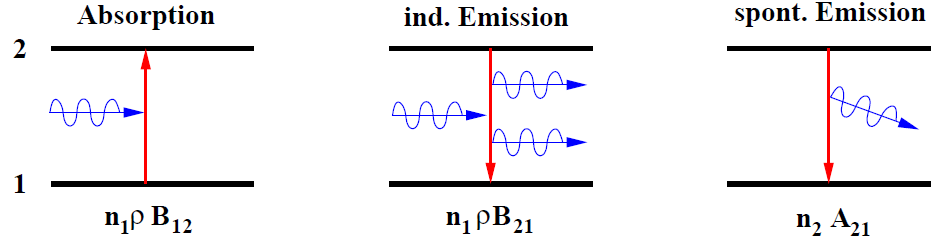
\includegraphics[]{images/schema_uebergaenge.png}
\label{fig:schema_uebergaenge}
\end{figure}

Die Wechselwirkung zwischen der Energiedichte $\rho$ der Strahlungsfeldes und des Zwei-Niveau-Systems ist durch die Gleichung
\begin{align}
 \dot{N}_\text{A}   & =n_1 \rho\left(\nu \right)B_{12}  &\text{Absorption} \\
 \dot{N}_\text{IE}  & =n_2 \rho\left(\nu \right)B_{21}  &\text{induzierte Emission} \\
 \dot{N}_\text{SE}  & =n_2 A_{21}                       &\text{spontane Emission} \\
\end{align}
mit den Einsteinkoeffizienten $A_{21}$, $B_{12}$ und $B_{21}$, die Übergangswahrscheinlichkeiten zwischen den Zuständen beschreiben, gegeben.

Aus diesen Gleichungen lassen sich, unter der Bedingung, dass keine Verluste ($n_1+n_2=$const.) auftreten, die Ratengleichungen für die Besetzungszahlen
\begin{align}
 \frac{d n_1}{d t}&=-n_1B_{12}\rho+N_2B_{21}\rho+n_2A_{21}\rho \\
 \frac{d n_2}{d t}&=-n_2B_{21}\rho+N_1B_{12}\rho-n_2A_{21}\rho
\end{align}
herleiten.

Damit das Strahlungsfeld kohärent und dauerhaft verstärkt wird, muss die stimulierte Emission häufiger auftreten als die spontane Emission. 
Nun sind die Zustände nach Maxwell-Boltzmann besetzt, sodass der Grundzustand viel stärker besetzt ist als der angeregte Zustand und die spontane Emission dominiert.
Um dies zu ändern, muss der angeregte Zustand häufiger besetzt sein. Dies wird durch eine Besetzungsinversion realisiert. 
Damit die Besetzungsinversion dauerhaft ist, muss die ganze Zeit Energie in das aktive Medium zugeführt werden. Dies wird auch Pumpen genannt.

Da die Verstärkung exponentiell mit der Länge des Laufwegs des Lichts durch das aktive Medium steigt, wird der Laserstrahl durch einen optischen Resonator mehrfach durch das aktive Medium geleitet.

\begin{figure}[h]
 \centering
 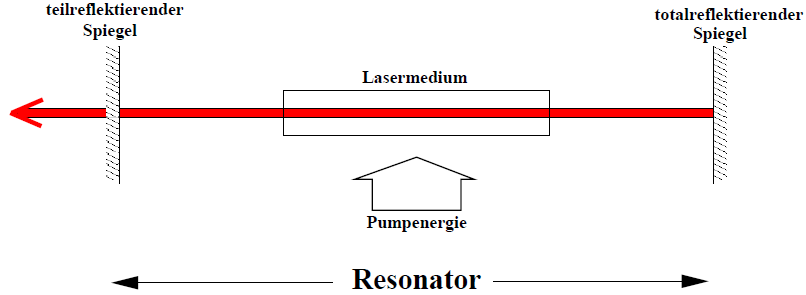
\includegraphics[]{images/schema_resonator.png}
\label{fig:schema_resonator}
\end{figure}

Wie in Abbildung \ref{fig:schema_resonator} dargestellt, besteht der optische Resonator aus zwei parallelen Spiegeln, von denen ein Spiegel teildurchlässig ist, um den Laserstrahl auszukoppeln.
Die Spiegel können dabei entweder nur planparallel oder nur sphärisch oder eine Kombination dieser beiden Typen sein.
Es sollten jedoch die Verluste durch die Spiegel geringer sein als die Verstärkung durch die angeregte Emission, damit ein angetriebenen Oszillator entsteht.
Um eine charakteristische Größe für diese optische Stabilität zu erhalten, wird der Resonatorparameter
\begin{align}
 g_i := 1- \frac{L}{r_i}
\end{align}
mit der Länge $L$ des Resonators und der Krümmungsradius $r_i$ des Spiegels eingeführt.
Die optische Stabilität ist dann für
\begin{align}
0 \le g_1 \cdot g_2 \le 1 
\label{eq:stabilitaet}
\end{align}
gegeben.

Da die Resonatorlänge $L$ viel größer als die Wellenlänge $\lambda$ sein soll, erfüllen viele Frequenzen die Resonzbedingungen für stehende Wellen. 
Diese $q$ Wellenlängen werden als longitudinale Mode bezeichnet. Es können auch transversalen Moden durch z.B. Spiegelunebenheiten oder Verkippungen entstehen.
In Anlehnung an einen Hohlleiter werden diese Moden $TEM_{lpq}$ genannt, wobei $l$ und $p$ die Knoten in x- und y- Richtung sind und als transversale Modenzahl bezeichnet werden.
$q$ ist die longitudinale Modenzahl und wird oft weg gelassen, da sie für die skalare Feldverteilung irrelevant ist.  

Die Feldverteilungen für einen konfokalen Resonator mit runden Spiegeln ist durch
\begin{align}
 E_{lpq} \propto \cos \left(l \phi \right) \frac{4\rho^ 2}{\left(1+Z^2 \right)^{0.5\cdot \left(1+l\right)}}L_{q}^{p}\left( \frac{4\rho^2}{1+Z^2} \right)\exp \left(-\frac{\rho^2}{1+Z^2}\right)
\cdot \exp \left\{-i \left[ \frac{\left(1+Z \right)\pi R}{\lambda} + \frac{\rho^2Z}{1+Z^2} - \left(l+2p+1\right)\left(\frac{\pi}{2}-\arctan \left(\frac{1-Z}{1+Z}\right) \right) \right] \right\}
\end{align}
\begin{align*}
\text{mit} \rho= \sqrt{\frac{2\pi}{R\lambda}} \text{und} Z=\frac{2z}{R}
\end{align*}
approximativ gegeben. Dabei ist $L^{q}_{p}\left(u\right) $ das dazugehörige Laguerre-Polynom.

Aus dieser Feldverteilung lässt sich die Intensitätsverteilung bestimmen. Die Intensitätsverteilung der $TEM_{00}$ Mode, die Mode mit der hösten Symmetrie und den geringsten Verlusten, ist durch die Gaußverteilung
\begin{align}
 I\left(r\right)=I_0\exp \left(-\frac{2r^2}{\omega^2}\right)
\end{align}
mit der Maximalintensität $I_0$ gegeben. Der Strahlradius $\omega$ ist durch den Abstand $z$ von der minimalen Strahltaille $\omega_0$ und der Strahldivergenz 
\begin{align}
 \theta = \frac{\lambda}{\pi}\omega_0
\end{align}
gegeben. Er lässt sich durch
\begin{align}
 \omega\left(z\right)=\omega_0\sqrt{1+\left(\frac{\theta z}{\omega}\right)}
\end{align}
bestimmen. 
\section{Durchführung}

\section{Auswertung}

\subsection{Überprüfung der Stabilitätsbedingung}
Zur Untersuchung der Stabilität des Lasers wurden zwei Konfigurationen von Spiegeln verwendet. Es wurden Spiegel mit Krümmungsradien r$_1=1\si{\meter}$ und r$_2=1.4\si{\meter}$ sowie r$_1=1\si{\meter}$ und r$_2=\infty\si{\meter}$, d.h. einem planaren Spiegel, verwendet. \\
Gemäß der Stabilitätsbedingung aus Gleichung \ref{eq:stabilitaet} wurden dann Graphen erstellt, an welchen die maximale Distanz L abzulesen ist. Diese sind in Abbildung \ref{fig:stab} zu sehen. \\
\begin{center}
	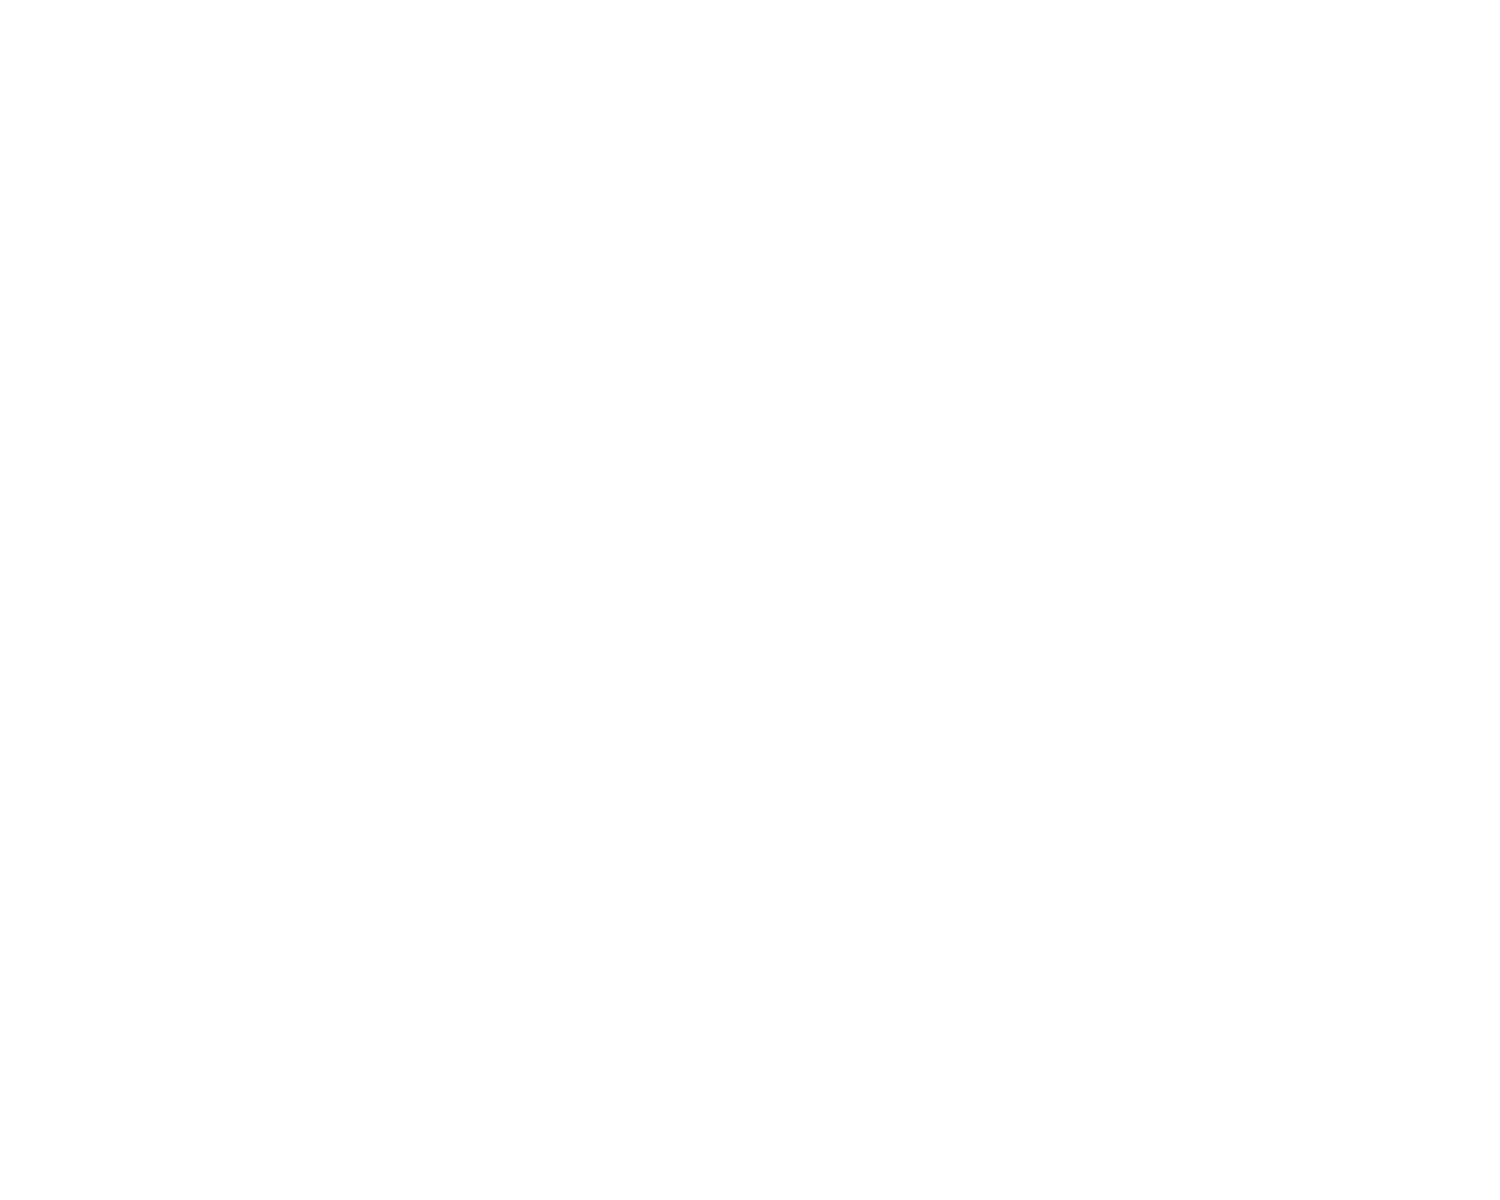
\includegraphics[width=\textwidth]{images/vorbereitung.pdf}
	\captionof{figure}{Stabilitätskurven des Lasers bei verschiedenen Linsenkonfigurationen}
	\label{fig:stab}
\end{center}
Aus der Abbildung können die beiden maximalen Längen L$_1=1.4\si{\meter}$ und L$_2=1\si{\metre}$ abgelesen werden. Im Experiment konnte nur die Kombination eines Spiegels mit Krümmungsradius r$=1.4\si{\metre}$ und eines planaren Spiegels verwendet werden. Die maximal erreichbare Resonatorlänge betrug dabei L$_{\text{max}}=1.34\si{\meter}$.

\subsection{Bestimmung der Wellenlänge des Lasers}
Zur Bestimmung der Wellenlänge des vom Laser emittierten Lichts wurden die Positionen von einem durch ein Gitter mit g=100$\frac{1}{\si{\milli\metre}}$ erzeugten Maxima aufgezeichnet. Diese Messwerte sind in Tabelle \ref{tab:maxima} dargestellt. \\
\begin{center}
	\begin{tabular}{|c|c|}
		\hline  & B$_1$ [$\mu$T] \\

	\end{tabular}
	\captionof{table}{Distanz der einzelnen Maxima vom 0. Maximum}
	\label{tab:mmaxima}
\end{center}


\subsection{Ausmessung der TEM00-Mode}

\section{Quellen}

\end{document}